\documentclass{../cs-classes/cs-classes}

\title{Extending Layer-wise Relevance Propagation using Semiring Annotations}
\author{
    \textbf{Antoine Groudiev}\\L3, DI, ENS
}
\date{}

\addbibresource{report.bib}
\graphicspath{{../cs-classes}{../images}}

\newcommand*{\K}{\mathbb{K}}
\newcommand*{\1}{\digitsbb{1}}
\newcommand*{\0}{\digitsbb{0}}

\begin{document}
\begin{abstract}
    Recently, neural networks allowed computers to solve numerous problems from diverse machine learning fields, such as natural language processsing and computer vision. Compared to traditional algorithms, machine learning models have proven both more successful and more difficult to interpret. Neural networks are considered as black boxes unable to easily explain themselves, that is justifying the reasons that led them to make a prediction. Layer-wise Relevance Propagation (LRP) is a technique that has been introduced to provide explanability by identifying the input features relevant to the output choice. In parallel, research in the databases field developed annotations techniques to compute provenance for queries. In this paper, we extend LRP propagation rules to semiring-based provenance annotations of the network, and implement semiring-based propagation rules for computer vision models of different scales.
\end{abstract}

\section{Introduction}
\subsection{Problem statement}
Deep neural networks have proven successful for solving with high accuracy machine learning problems. The expressivity of the class of functions generated by neural networks, combined with the relative simplicity of their training, make such models versatile tools to learn the relationship between the inputs and outputs of a dataset.

However, this versatility comes at the cost of poor interpretability: a neural network simply represents a function from one high-dimensional space to another, but provides no justification nor explanation for a given execution. If metrics such as the accuracy over a testing set provide confidence in the fact that the model is able to correctly classify inputs similar to the training set, no guarantee is given that the model generalizes well. Real-world examples show that networks can overfit the input data, or even take shortcuts instead of learning the intended solution \cite{shortcuts}. For the user to have confidence in its predictions, a neural network should therefore be able to highlight the patterns in the input data that it actually learned.

\subsection{Layer-wise Relevance Propagation}
Layer-wise Relevance Propagation (LRP) \cite{bach-2015} has been introduced as a technique to explain an execution of a neural network. LRP is a procedure propagating the output of the function backward in the network, using diverse rules to compute the \emph{relevance} of a neuron depending on the relevances of the neurons of the upstream layer. LRP introduces the notion of \emph{relevance score} for a neuron, intuitively quantifying the contribution of this neuron to the classification of final classification. A high relevance score indicates that the neuron led to the activation of the considered output; a negative relevance score represents neurons that increased the activation of another output neuron instead of the one considered.

\begin{figure}[H]
    \centering
    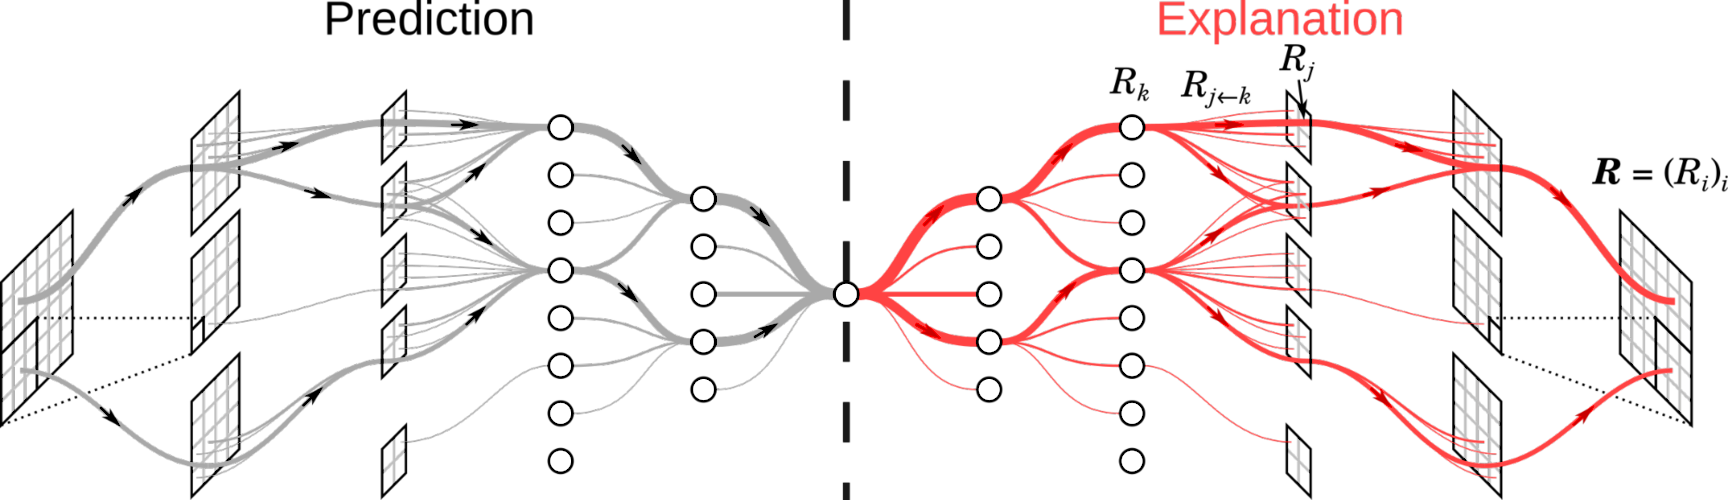
\includegraphics[width=.8\textwidth]{LRP.png}
    \caption{Illustration of LRP. The leftmost part corresponds to the forward pass, while relevance propagation is visualized in the rightmost part.\protect\footnotemark}
\end{figure}
\footnotetext{Figure adapted from \href{https://www.hhi.fraunhofer.de/en/departments/ai/technologies-and-solutions/layer-wise-relevance-propagation.html}{\say{Layer-wise Relevance Propagation}} -- Fraunhofer Institute for Telecommunications}

\subsubsection{Setup and notations}
In the following, we consider a deep neural network used for a classification task. We assume that it uses the rectifier activation function\footnote{That is $\ReLU(x)=\max(0, x)$, where ReLU stands for \emph{Rectified Linear Unit}.}, which is the case in most applications. To ease the notation, we will not consider biases but instead assume that the first neuron of each layer represents the bias. 

Let $L$ be the number of layers of the network, including the input and output layers. We denote by $\left(a^{(l)}_k\right)_k$ the activations of the network. Notably, $\left(a^{(1)}_k\right)_k$ is the input data, and $\left(a^{(L)}_k\right)_k$ is the ouput prediction. We denote by $\left(w^{(l)}_{j, k}\right)_{j, k}$ the weights connecting the $l$-th layer to the $(l+1)$-th layer. To simulate the biases using only weight matrices, we set:
\begin{equation*}
    \forall l\in\iset{1}{L}, \quad a^{(l)}_0 = 1
\end{equation*}
and we define $w^{(l)}_{0, k}$ to be the bias of the $k$-th neuron of the $(l+1)$-th layer. The forward propagation rule of a deep rectifier network is therefore:
\begin{equation}
    \forall l\in\iset{1}{L-1}, \forall k, \quad a^{(l+1)}_k = \ReLU\left(\sum_{j}a^{(l)}_j w^{(l)}_{j, k}\right) = \max\left(0, \sum_{j}a^{(l)}_j w^{(l)}_{j, k}\right)
\end{equation}

We denote by $R^{(l)}_j$ the relevance of the $j$-th neuron of the $l$-th layer. We assume that the output layer represents a one-hot encoding, that is that the belonging of the input to the $i$-th class is represented by an output vector is of the form $(0, \dots, a^{(L)}_i, \dots, 0)$, where the only non-null coefficient is in the $i$-th position. Finally, we denote by $y$ the label of a classified input. To the label $y=i$ is associated the output vector $(0, \dots, a^{(L)}_i, \dots, 0)$.

\subsubsection{Propagation rules}
Relevance scores are initialized for the output layer, and are set to the output activation for the correct class, that is:
\begin{equation}
    R^{(L)}_i = \begin{cases*}
        a^{(L)}_i & if $i = y$\\
        0 & otherwise
    \end{cases*}
\end{equation}

The simplest LRP rule is called LRP-0. It propagates the relevance to a neuron of the lower layer proportionnaly to its contribution to each of the neuron of the next layer:
\begin{equation}
    R^{(l)}_j = \sum_{k}\frac{a^{(l)}_jw^{(l)}_{j, k}}{\sum_{j'}a^{(l)}_{j'}w^{(l)}_{j', k}} R^{(l+1)}_k
\end{equation}
The denominator $\sum_{j'}a^{(l)}_{j'}w^{(l)}_{j', k}$ guarantees a conservation property, that is that for any layer $l$:
\begin{equation*}
    \sum_j R^{(l)}_j = \sum_k R^{(l+1)}_k
\end{equation*}
This allows to keep the information regarding the total activation of the final layer.

\begin{figure}[H]
    \centering
    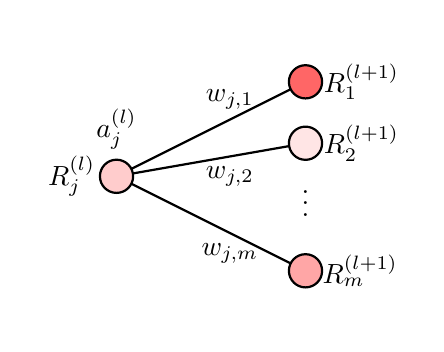
\begin{tikzpicture}[scale=.6]
        \draw[thick] (0,0) -- (4, 2) node[above=.12, pos=.6] {$w_{j,1}$};
        \draw[thick] (0,0) -- (4, .7) node[below, pos=.6] {$w_{j,2}$};
        \draw[thick] (0,0) -- (4, -2) node[below=.12, pos=.6] {$w_{j,m}$};

        \node at (0, 1) {$a_j^{(l)}$};
        \draw[thick, fill=red!20,circle,minimum size=15] (0, 0) circle (10pt) node[left] {$R_j^{(l)}$};

        \draw[thick, fill=red!60,circle,minimum size=15] (4, 2) circle (10pt) node[right=.2] {$R_1^{(l+1)}$};
        \draw[thick, fill=red!10,circle,minimum size=15] (4, .7) circle (10pt) node[right=.2] {$R_2^{(l+1)}$};
        \node at (4, -.4) {$\vdots$};
        \draw[thick, fill=red!35,circle,minimum size=15] (4, -2) circle (10pt) node[right=.2] {$R_m^{(l+1)}$};
    \end{tikzpicture}
    \caption{Node-level illustration of relevance propagation.}
\end{figure}

The application of this simple rule can lead into noisy results that do not scale well. An overview of variations of LRP-0 is provided by \cite{montavon-lrp}; not all rules are suitable for all layers. Complex deep neural networks architectures benefit from enhanced rules such as LRP-$\epsilon$ or LRP-$\gamma$, which provide more stable explanations.

Notably, the input layer must be handled using a different rule, since it does not receive its input from ReLU activations, but directly from the input data. The $z^\mathcal{B}$ rule is used in \cite{montavon-lrp} to propagate from layer 2 to 1 (input layer):
\begin{equation}
    R^{(1)}_j = \sum_{k} \frac{x_kw_{j, k} - l_jw^+_{j, k} - h_jw_{j, k}^-}{\sum_{j'}x_kw_{j', k} - l_jw^+_{j', k} - h_jw_{j', k}^-} R^{(2)}_k
\end{equation}
where $(\cdot)^+=\max(0, \cdot)$, $(\cdot)^-=\min(0, \cdot)$. The parameters $l_i$ and $h_i$ respectively define the theoretical minimum and maximum values of the inputs $x_i$. For instance, we might have $l_i=0$ and $h_i=255$ for pixels over 8 bits.

\subsubsection{LRP results and pertinence}
Previous works (\cite{bach-2015}, \cite{montavon-lrp}), as well as the methods that we will introduce later on, were experimentaly tested on models trained over two datasets: fully-connected networks trained on the MNIST handwritten digits dataset \cite{mnist-dataset}, and deep convolutional networks pre-trained on the ImageNet visual database such as VGG-16 \cite{vgg}.

\autoref{fig:mnist-lrp} shows relevance for a simple model: a fully-connected deep rectifier network with layers of sizes $28\times28$, $300$, $100$ and $10$, trained on the MNIST dataset. Pixels highlighted in red have a positive relevance while blue pixels have a negative relevance. As expected, the relevant pixels to classify this image as a \texttt{0} are the white pixels in the input image.

\begin{figure}[H]
    \centering
    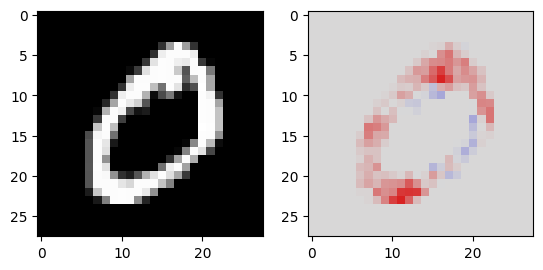
\includegraphics[width=.5\textwidth]{mnist-lrp.png}
    \caption{Input image and pixel-wise explanation of the output neuron \texttt{0}}
    \label{fig:mnist-lrp}
\end{figure}

\autoref{fig:castle-lrp} provides a visualization for a more complex example, an execution of the VGG-16 network over a $224\times224$ image. 
\begin{figure}[H]
    \centering
    \begin{minipage}[c]{.49\textwidth}
        \centering
        
\includegraphics[width=.65\textwidth]{castle.jpg}
    \end{minipage}
    \hspace*{-2.5cm}
    \begin{minipage}[c]{.49\textwidth}
        \centering
        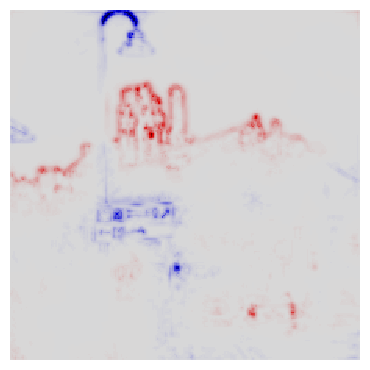
\includegraphics[width=.65\textwidth]{castle-lrp.png}
    \end{minipage}
    \caption{Input image and relevance for the class "\texttt{castle}" of the VGG-16 network}
    \label{fig:castle-lrp}
\end{figure}
Note that the castle part of the image is highlighted in red as intended. Furthermore, both the street sign and the street light have strong negative relevance; those two objects correspond to other classes of the ImageNet dataset (\texttt{street sign (919)} and \texttt{traffic light (920)}). Those two elements of the image would have positive relevance for LRP starting from the output neurons \texttt{919} and \texttt{920}.

% TODO: double MNIST?

\subsection{Semiring-based provenance annotations}
In parallel, the notion of data provenance in databases theory developed formal solutions to a similar problem to ours. Data provenance aims at \emph{explaning} a query by highlighting the tuples in the original database that led to the presence of a certain tuple in the query result. If contexts are different, deep neural networks explanation and data provenance share the same general setup: identifying a subset of the input that directly implied a certain output.

A framework to approach data provenance is \emph{provenance semirings}, introduced in \cite{green-2007}, annotates tuples using abstract elements of a semiring and apply semiring operations to the tuples appearing in the query. As the query is executed, information about the provenance of the intermediate results is aggregated, resulting in an abstract formula that can be concretized by substituting abstract elements and operations by a concrete semiring. Similarly, in the context of graph databases, edges can be annotated to derive a variety of properties of the query result. \cite{ramusat-prov}

In the following, we provide a mathematical definition of a semiring as well as semiring examples suited for the application to deep neural networks.

\begin{definition}[Semiring]
    A \emph{semiring} is an algebraic structure generalizing the notion of rings. A semiring $(\K, \oplus, \otimes, \0, \1)$ is composed of a set $\K$, binary operators $\oplus$ and $\otimes$ such that $\otimes$ distributes over $\oplus$, verifying the following properties:
    \begin{itemize}
        \item $(\K, \oplus, \0)$ is a commutative monoid
        \item $(\K, \otimes, \1)$ is a monoid such that $\0$ is absorbing
    \end{itemize}
\end{definition}

\begin{example}
    $(\R, +, \times, 0, 1)$ is a semiring. While it has no direct interpretation is the context of databases, we will see that is corresponds to the basic real-valued LRP.
\end{example}

\begin{example}[Boolean semiring]
    $(\B, \lor, \land, \bot, \top)$ where $\B:=\{\bot, \top\}$ is a semiring. Its use in databases provenance interprets as the existence of a path between two vertices, using edge weights as the number of different paths between two adjacent vertices. 
\end{example}

\begin{example}[Counting semiring]
    $(\mathbb{N}, +, \times, 0, 1)$ is a semiring. For a non-cyclic graph database, its use allows to compute the total number of paths between two vertices, using edge weights as the number of different paths between two adjacent vertices.
\end{example}

\begin{example}[Viertbi semiring]
    $([0, 1], \max, \times, 0, 1)$ is a semiring. For a non-cyclic graph database where the annotations are interpreted as a \say{confidence} measure, its use allows to compute the confidence score of the result of a query.
\end{example}

\section{Extending LRP using Semiring Annotations}
We aim at extending Layer-wise Relevance Propagation by annotating the computational graph of a neural network with semiring elements.

\subsection{Semiring generalization of the LRP rules}
LRP rules all inherit the same structure, in which the relevance of a pixel can be expressed as the weighted sum of the relevance of pixels of the next layer:
\begin{equation}
    R_j^{(l)} = \sum_k d_{j, k}^{(l)} \cdot R_k^{(l+1)}
    \label{eq:general-lrp}
\end{equation}
where the $d_{j,k}^{(l)}$ are some coefficients proportional to the extent to which neuron $j$ of the $l$-th layer has contribued to make neuron $k$ of the $(l+1)$-th layer relevant.

\autoref{eq:general-lrp} is the special real-valued case of a more general rule. Let $(\K, \oplus, \otimes, \0, \1)$ be a semiring, and $(\Theta^{(l)})_l$ be annotation functions, associating to each matrix of coefficients $d^{(l)}$ a matrix of semiring elements $\Theta^{(l)}(d)$. In particular, note that $d_{i,j} \mapsto \Theta^{(l)}(d)_{i,j}$ does not need to be a mapping: to identical coefficients can be associated different annotations. In the following examples, we will mostly use element-wise annotations functions of the form $\R\longrightarrow\K$.

We call $\K$-relevance for output neuron $y$ the quantity $R\in\K$ inductively defined by:
\begin{equation}
    R^{(L)}_i := \begin{cases*}
        \1 & if $i = y$\\
        \0 & otherwise
    \end{cases*}
    \label{eq:semiring-lrp-init}
\end{equation}
and
\begin{equation}
    R^{(l)}_j := \bigoplus_{k}\Theta^{(l)}(d)_{j,k} \otimes R^{(l+1)}_k
    \label{eq:semiring-lrp-rec}
\end{equation}
Note that choosing $(\R,+,\times,0,1)$ as a semiring and $\Theta^{(l)}=x\mapsto x$ retrieves classical LRP up to a multiplicative factor of $a_i^{(L)}$ on each layer (which does not appear on the semiring initialization).

Equations \ref{eq:semiring-lrp-init} and \ref{eq:semiring-lrp-rec} can be intuitively interpreted in two ways. Firstly, they can be seen as the abstraction of an LRP computation using formal semiring elements. Computing $\K$-relevance for an execution of the network results in an abstract formula in terms of elements of $\K$ and operations $\oplus$ and $\otimes$. While this might be useful in the context of graph provenance, visualizing abstract formulas is difficult because of the size of computational graphs associated to neural networks. Furthermore, the general structure of the formulas is always the same for a specific model, since neural networks usually have very simple computational graphs structures. 

Therefore, a second approach that fits the graph properties of neural networks is to interpret semiring LRP as operations on an annotated circuit, similarly to \cite{senellart2018provenance}. For instance, in the case of the boolean semiring, computing $\B$-relevance consists in taking for each node the logical conjunction of the annotations of its outgoing edges.
% TODO: add boolean circuit example figure

Similarly to the implementation of provenance in databases by tools such as ProvSQL \cite{provsql}, we implemented a Python module on top of PyTorch\footnote{\href{https://pytorch.org}{\texttt{https://pytorch.org}}}, providing an interface to compute $\K$-relevance for any custom semiring $\K$.


\subsection{Results over the MNIST dataset}
We provide experimental results of the implementation of semiring-based LRP. In the following, we use the same fully-connected network as in \autoref{fig:mnist-lrp}, with layers of sizes $28\times28$, $300$, $100$ and $10$ and trained on the MNIST dataset.
\subsubsection{Boolean Semiring}
Boolean relevance can be computed using the boolean semiring $(\B=\{\bot, \top\}, \lor, \land, \bot, \top)$, and an element-wise annotation function $\Theta$ of the form:
\begin{equation}
    \begin{aligned}
        \Theta: \R&\longrightarrow \B\\
        x&\longmapsto \begin{cases*}
            \top & if $x\geq\theta$\\
            \bot & otherwise
        \end{cases*}
    \end{aligned}
\end{equation}
where $\theta$ is a hyperparameter called the threshold. A higher threshold reduces the number of $\top$ coefficients, ultimately reducing the number of input neurons having a relevance equal to $\top$. Choosing $\theta=10^{-9}$ filters out null and negative contributions to the output while maintaining a sufficient amount of activated inputs for visualization.

\begin{figure}[H]
    \centering
    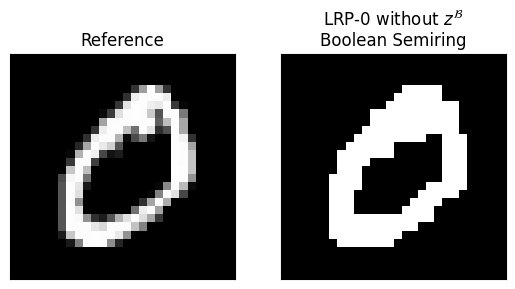
\includegraphics[width=.5\textwidth]{boolean.png}
    \caption{Input image and $\B$-relevance for the output neuron \texttt{0} for $\theta=10^{-9}$}
\end{figure}

The full propagation equation becomes:
\begin{equation}
    R^{(l)}_j := \bigvee_{k}\Theta\left(\frac{a_j\cdot w_{j, k}}{\sum_{j'}a_{j'}\cdot w_{j', k}}\right) \land R^{(l+1)}_k
    \label{eq:boolean-lrp}
\end{equation}

$\B$-relevance provides a higher level explanation, highlighting large zones of the input image which contribute the most to the final classification.
Naturally, information about nuances in the contribution is lost. Intuitively, activated pixels (input neurons with relevance $\top$) are neurons such that there exists a \say{relevant} path from this neuron to the output neuron of the class \texttt{0}. A relevant path is a path in which all edges have a weight higher than the threshold $\theta$. While this condition might seem quite restrictive, note that computation graphs for neural networks are densely connected: there is $784\times300\times100=23\,520\,000$ different paths connecting one input pixel to the output neuron of the class \texttt{0}.

\subsubsection{Counting Semiring}
The counting semiring $(\mathbb{N}, +, \times, 0, 1)$ extends boolean relevance by enumerating the number of relevant paths starting from each input pixel. Its element-wise annotation function $\Theta$ is mostly identical:
\begin{equation}
    \begin{aligned}
        \Theta: \R&\longrightarrow\N\\
        x&\longmapsto \begin{cases*}
            1 & if $x\geq\theta$\\
            0 & otherwise
        \end{cases*}
    \end{aligned}
\end{equation}
but operations $+$ and $\times$ bring more expressivity to the framework, bringing more nuance in the highlighted zones.

\begin{figure}[H]
    \centering
    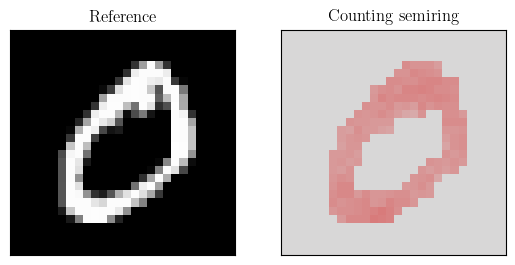
\includegraphics[width=.5\textwidth]{counting.png}
    \caption{Input image and $\N$-relevance for the output neuron \texttt{0} for $\theta=10^{-9}$.\\ Highest relevance is 2098.}
\end{figure}

The full propagation equation becomes:
\begin{equation}
    R^{(l)}_j := \sum_{k}\Theta\left(\frac{a_j\cdot w_{j, k}}{\sum_{j'}a_{j'}\cdot w_{j', k}}\right) \times R^{(l+1)}_k
    \label{eq:counting-lrp}
\end{equation}

\subsubsection{Viterbi Semiring}
The Viterbi semiring $([0, 1], \max, \times, 0, 1)$ replaces the $+$ of the classical real semiring by a $\max$. In a context where neurons can have the same weighted sum of relevance, taking the maximum of the relevance emphasizes the most important neurons, giving a more contrasted visualization than classical LRP. 
\begin{figure}[H]
    \centering
    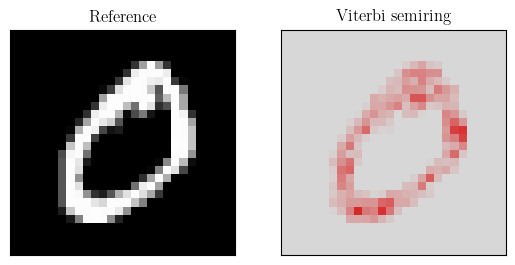
\includegraphics[width=.5\textwidth]{viterbi.png}
    \caption{Input image and $[0, 1]$-relevance for the output neuron \texttt{0}}
\end{figure}
To ensure that values belong to the $[0, 1]$ set, the following rule is used:
\begin{equation}
    R^{(l)}_j = \max_k \underbrace{\left(\frac{\left|a_j\cdot w_{j, k}\right|}{\max_{j'} \left|a_{j'}\cdot w_{j', k}\right|}\right)}_{\in[0, 1]} \cdot R^{(l+1)}_k
\end{equation}
In practice, a small amount such as \texttt{1e-9} can be added to the denominator to prevent from dividing by zero in the case where each $|a_{j'}\cdot w_{j',k}|$ is null.

\section{Handling Convolutional Neural Networks}
If LRP rules are well-suited for simple, feedforward neural networks, most use cases of explanations occur with larger models, namely deep convolutional neural networks (CNNs). We explain how previously introduced rules can be adapted to CNNs, and provide visualization examples for the VGG-16 model.

\subsection{Computing relevance for convolutional layers}
% TODO: explain CNN forward pass somewhere?
Convolutional layers are special types of linear layers, in which an output neuron of a layer does not depend on every single neuron from the input. While in a rule of the form
\begin{equation*}
    R_j^{(l)} = \sum_k d_{j, k}^{(l)} \cdot R_k^{(l+1)}
\end{equation*}
the sum $\Sigma_k$ relates to every neuron of the output layer, the neuron $j$ might have no influence at all on most of the neurons in this sum. Therefore, we can restrict the sum to only neurons of the output layer which depend on the $j$-th neuron of the input layer. This can be seen in LRP rules, since the coefficients $d_{j, k}^{(l)}$ are proportional to $w_{j,k}$, which is null if there is no connection between neurons $j$ and $k$. 

If applying directly the formula to convolutional layers is theoretically possible, it is prohibitely expensive to do so in practice. Two methods allow to efficiently compute relevance for convolutional layers. We will first review an efficient gradient-based approach, that requires automatic differentiation; secondly, we will propose a slower method that can be used without depending on the gradient computation.

\subsubsection{Gradient expression of LRP}
Classical LRP rules can be easily and efficiently implemented. A general rule encapsulating LRP-0/$\epsilon$/$\gamma$ can be written as:
\begin{equation}
    R_j^{(l)} = \sum_k\frac{a_j\cdot\rho(w_{j,k})}{\epsilon+\sum_{j'}a_{j'}\cdot{\rho(w_{j',k})}} \cdot R_k^{(l+1)}
\end{equation}
where $a=a^{(l)}$, $w=w^{(l)}$. Four steps, described in \cite{montavon-lrp}, allow for an efficient and effortless computation of relevance:
\begin{equation}
    \begin{aligned}
        \textstyle\forall k: z_k &= \epsilon + \sum\nolimits_{j'}a_{j'}\cdot\rho(w_{j',k})\\
        \forall k: s_k &= R_k / z_k\\
        \forall j: c_j &= \sum\nolimits_k\rho(w_{j',k})\cdot s_k\\
        \forall j: \!R_j &= a_j\cdot c_j
    \end{aligned}
\end{equation}

These steps provide two majors benefits. Firstly, it allows for the costly divisions by $z_k$ to be performed only once per $k$, independently of $j$. Secondly, the third step can be expressed as the computation of a gradient:
\begin{equation}
    c_j = \left[\nabla\left(\sum\nolimits_k z_k(a^{(l)})\cdot s_k\right)\right]_j
\end{equation}
where the gradient $\nabla$ is taken with respect to the vector $a^{(l)}$ and where the $s_k$ are treated as constants. This allows for a simple and efficient implementation, since the gradient can be computed using automatic differentiation: the high-level code is not only concise (two lines of PyTorch code), but also effortlessly generalizable  to any layer implementing backward pass, and highly optimized using GPU operations.

\subsubsection{Implementing LRP without automatic differentiation}
While the gradient-based expression is convenient for classical LRP, it does not allow for the overloading of sum and product operations, making it impossible to use with a semiring of our choice. To overcome this limitation, we explicitely derive the dependency between input and output neurons of the convolutional layer, resulting in less flexible code. 

Notice that the sum of contributions of one neuron to the output can be expressed as a convolution over the output. That is, in a formula of the form:
\begin{equation*}
    R_j^{(l)} = \sum_k \frac{z_{j,k}}{\sum_{j'}z_{j',k}} \cdot R_k^{(l+1)}
\end{equation*}
the sum in the denominator, $\sum_{j'}z_{j',k}$, can be expressed as a forward pass of the convolutional layer, that is a convolution over the input; in contrast, the main sum, $\sum_k$, can be expressed as a convolution over the output relevance.

% TODO

\subsubsection{Other CNN layers}
Most deep convolutional neural networks contain other special layers. We provide a general description of how these were handled in our experiments on the VGG-16 model.

\paragraph*{Average Pooling}
Such layers can be seen as convolutional layers with fixed weights, in which each weight of the kernel is identical. In practice, most average pooling layers are used with a stride equal to the kernel size $K$, creating no overlapping. Therefore, the propagation rule for average pooling layers can be simplified as:
\begin{equation}
    R^{(l)}[i][j] := \Theta(d_{i,j}) \otimes R^{(l+1)}[i/K][j/K]
\end{equation}
where $K$ is the kernel size.

\paragraph*{Batch Normalization Layers}
At test time, normalization layers act as a linear operatioin, and can therefore be fused with the previous linear layer. LRP and semiring-based LRP can then be applied directly to the fused layer.

\subsection{Results for the VGG-16 network}
We conducted experiments on the VGG-16 network \cite{vgg}, trained on the ImageNet-1K dataset, containing 1\,281\,167 images from 1\,000 classes. Its very deep architecture makes it a challenging model for relevance propagation, since minor changes in the deeper layers can ruin the visualization of the first layers.
\begin{figure}[H]
    \centering
    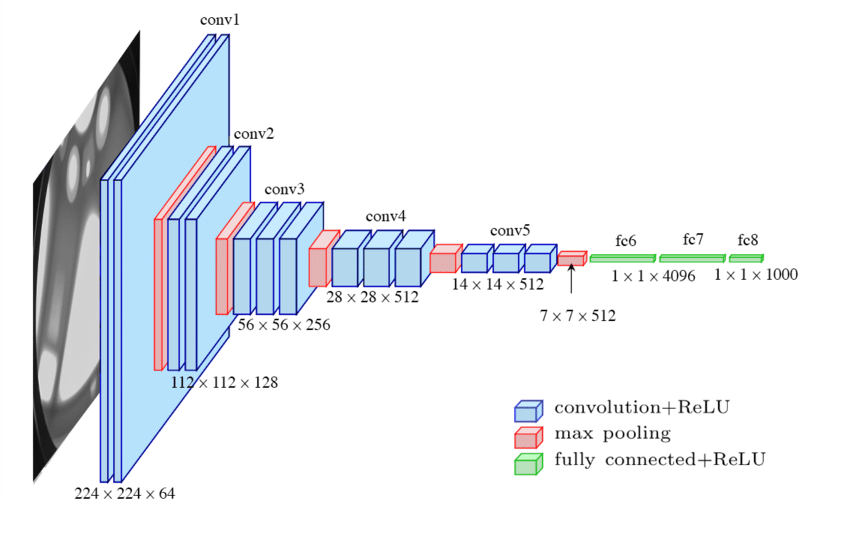
\includegraphics[width=.6\textwidth]{vgg-architecture.png}
    \caption{Architecture of the VGG-16 network.\protect\footnotemark}
\end{figure}
\footnotetext{Figure reproduced from Max Ferguson et al., `Automatic localization of casting defects with convolutional neural networks.' (2017)}
A necessary ajustement compared to the simpler fully-connected neural networks is to be able to choose a different annotation function for each layer. Instead of using the same $\Theta$ at every layer, a family of functions $(\Theta^{(l)})_l$ is used. In practice, since we used threshold-based annotation functions, this means that each layer will have a different threshold. We discuss the choice of thresholds and the correlation to other parameters of the network in \autoref{seq:thresholds-choice}.

\subsubsection{Boolean semiring}
$\B$-relevance over VGG-16 is coherent with results on the MNIST dataset: it specifies a main zone of importance in the image, similarly to explainations of tools such as Grad-CAM \cite{gradcam}.
\begin{figure}[H]
    \centering
    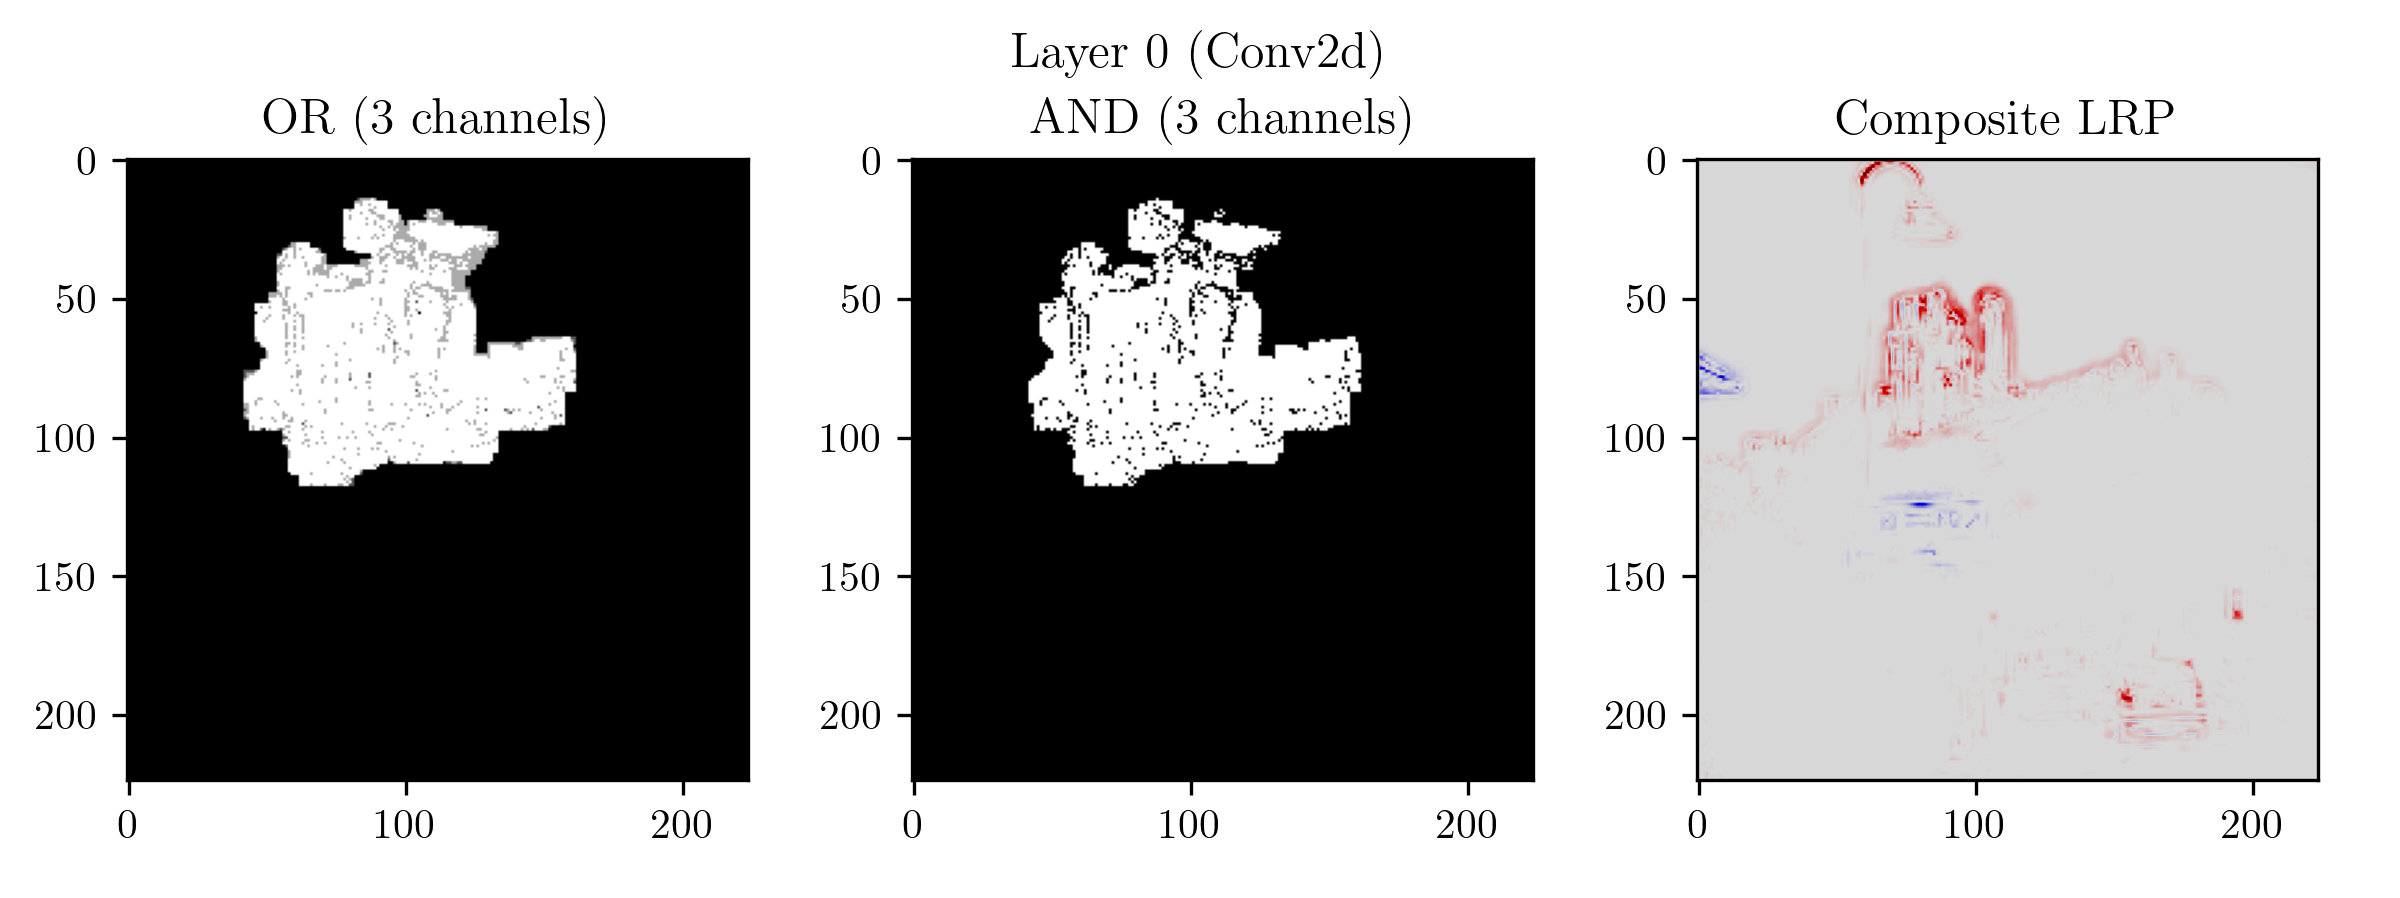
\includegraphics[width=.9\textwidth]{vgg-boolean.png}
    \caption{$\B$-relevance of the class \texttt{castle}. The input layer having three channels (R, G, B), they are aggregated using OR/AND operations.}
    \label{fig:vgg-boolean}
\end{figure}
While classical LRP provides a more precise explanation by focusing on the contours of the relevant object, $\B$-relevance selects all the pixels of the object, including its center.

\subsubsection{Counting semiring}
Counting semiring produces an explanation qualitatively similar to classical LRP. 
\begin{figure}[H]
    \centering
    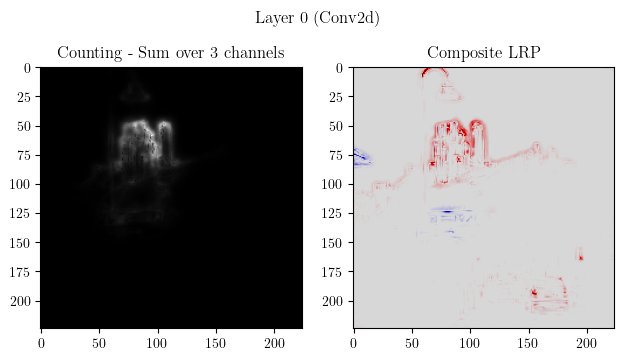
\includegraphics[width=.65\textwidth]{vgg-counting.png}
    \caption{$\N$-relevance of the class \texttt{castle}. The three channels are aggregated\\ using a sum, like for composite LRP.}
\end{figure}

\subsubsection{Viterbi semiring}

\subsection{Thresholds choice}
\label{seq:thresholds-choice}
Equations such as \ref{eq:boolean-lrp} and \ref{eq:counting-lrp} introduce thresholds which must be ajusted to provide meaningful explanation. Selecting such parameters optimally requires a proper definition of explanation quality, which is a separate research domain \cite{samek2016evaluating}. Nevertheless, only some ranges of threshold values guarantee a final result that is humanly interpretable. Threshold values that are too high result in visualizations containing little to no information; relevance is \say{lost} in the deepest layers and only a few input neurons are marked as relevant. Threshold values that are too low result in over-saturated visualizations; for instance, boolean relevance selects most neurons as relevant, loosing meaningful information in the amount of activated pixels.

We propose threshold values, used in \autoref{fig:vgg-boolean}, that offer a balanced explanation. Modifiying these values by small amounts allow the user to choose between a more precise or more general explanation.
\begin{figure}[H]
    \centering
    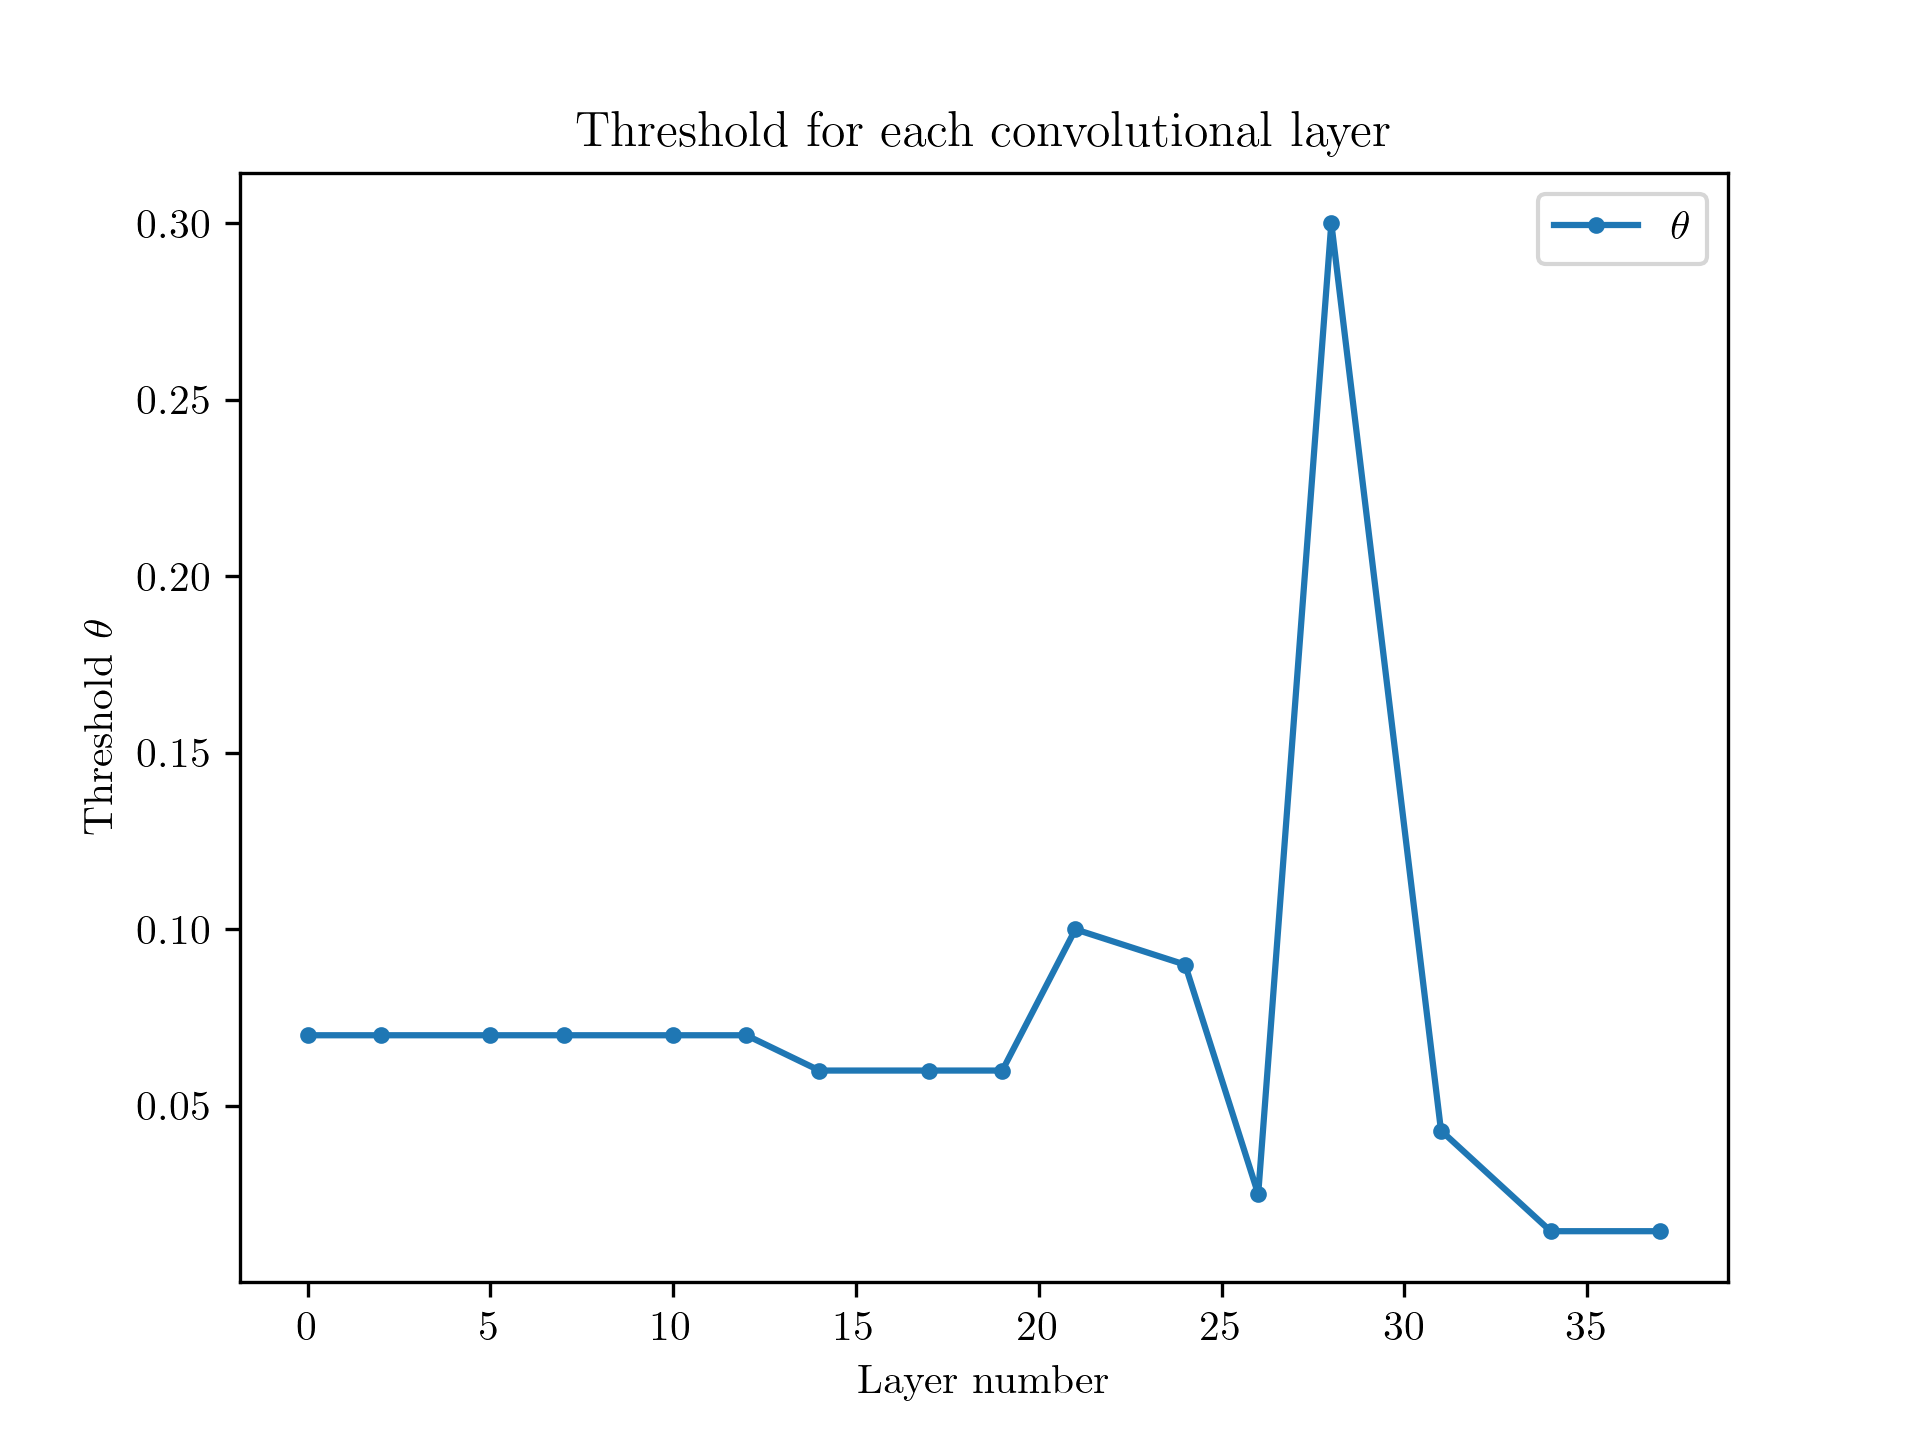
\includegraphics[width=.6\textwidth]{threshold-graph.png}
    \caption{Variation of the threshold of convolutional layers used to compute $\B$-relevance}
\end{figure}

While those parameters were handpicked, they appear to be correlated to parameters of the layers.

% TODO

\section{Applications}
Finally, we explore multiple applications of semiring-based LRP, going beyond the scope of simple execution-wise explanations. While LRP was intended as a tool to interpret a single execution of the network, we believe that averaging relevance scores of neurons over multiple executions can produce a meaningful metric of the \say{importance} of each neuron. Through three applications, we put forwards both qualitative and quantitative arguments supporting this view.

\subsection{Image mask computation}
\begin{figure}[H]
    \centering
    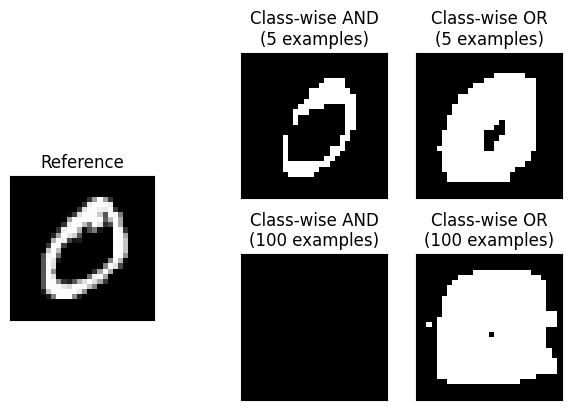
\includegraphics[width=.5\textwidth]{boolean-mask.png}
    \caption{Class-wise mask for $\B$-relevance of the class \texttt{0}}
\end{figure}

\begin{figure}[H]
    \centering
    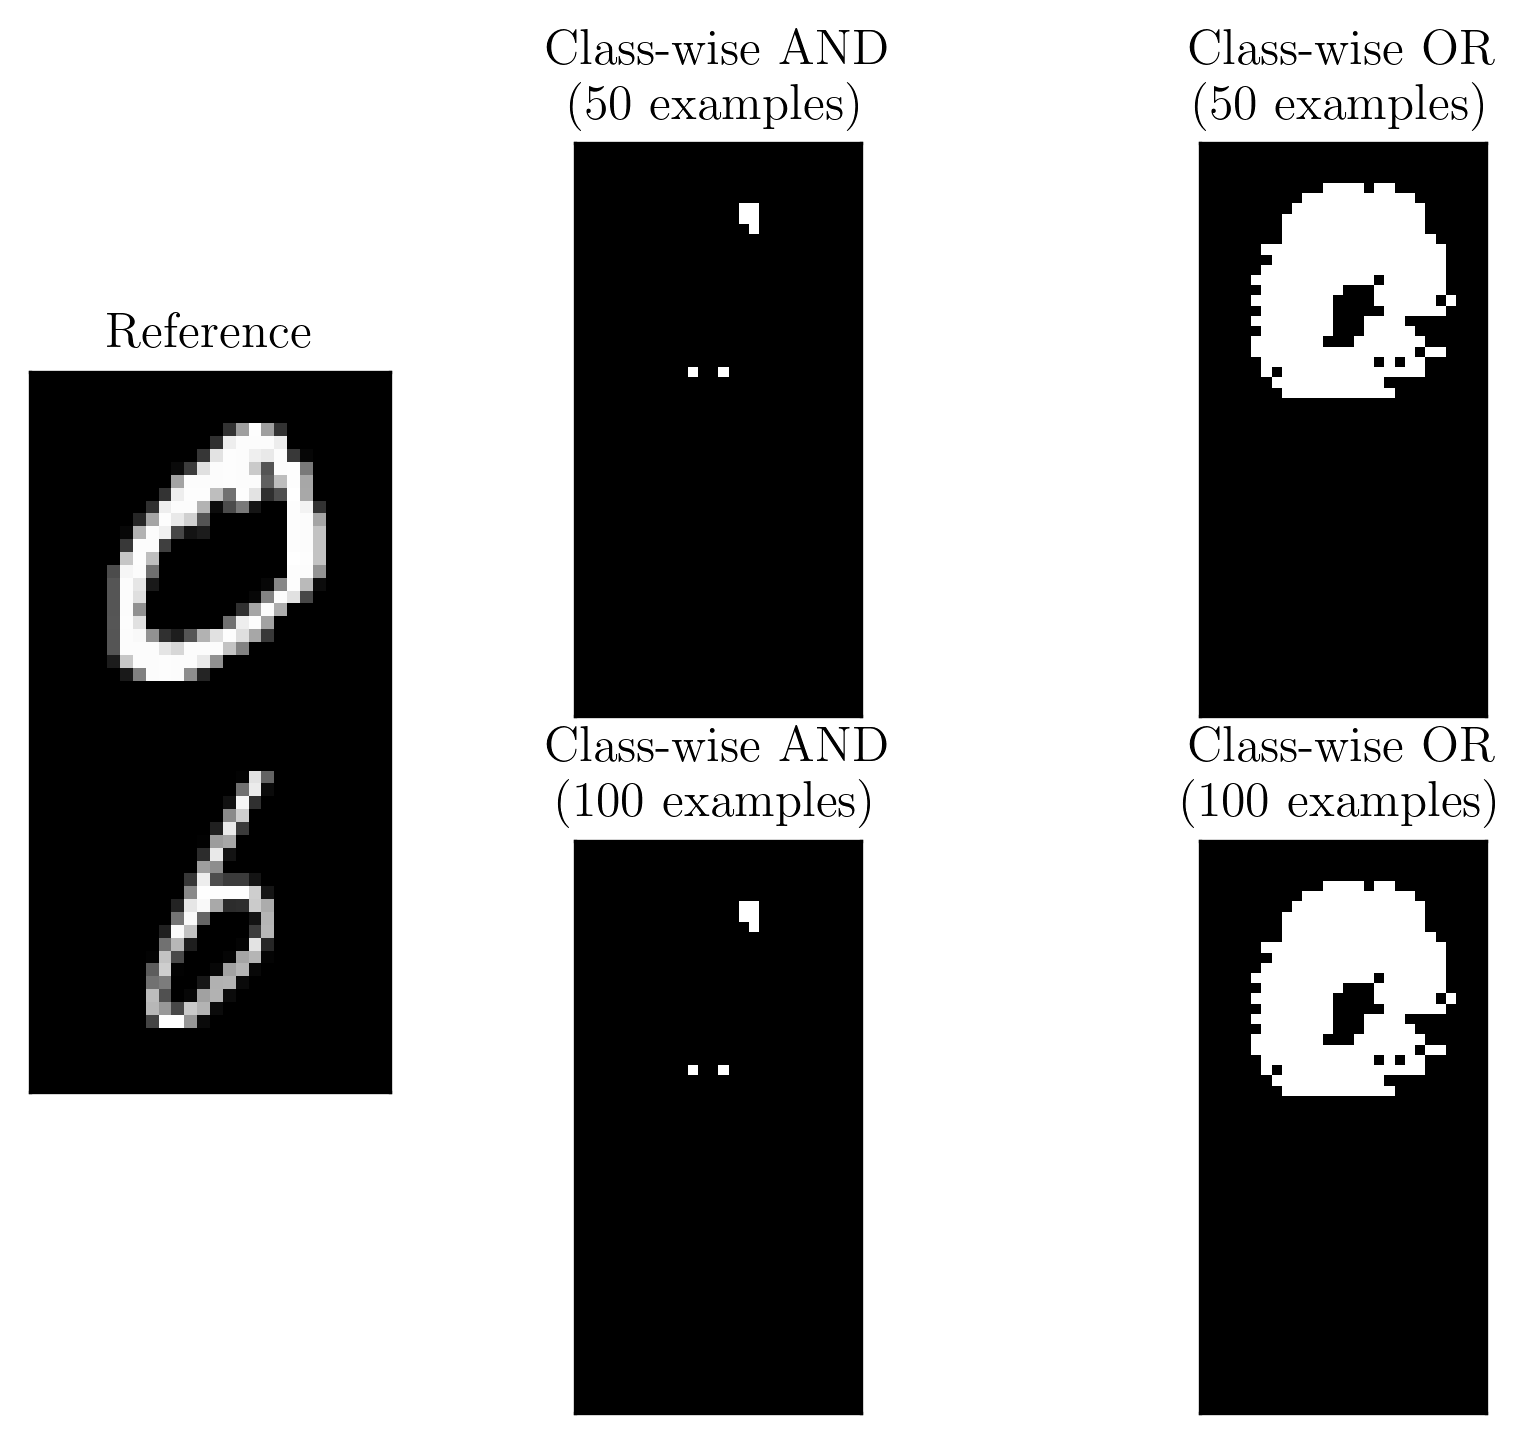
\includegraphics[width=.5\textwidth]{dmnist-boolean-mask.png}
    \caption{Class-wise mask for $\B$-relevance of the class \texttt{0}}
\end{figure}

\begin{figure}[H]
    \centering
    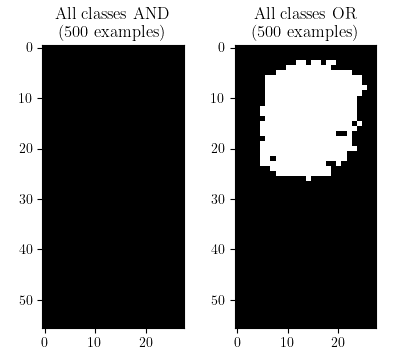
\includegraphics[width=.5\textwidth]{dmnist-all-classes.png}
    \caption{Class-wise mask for $\B$-relevance of the class \texttt{0}}
\end{figure}

% TODO: add double MNIST

% \begin{figure}[H]
%     \centering
%     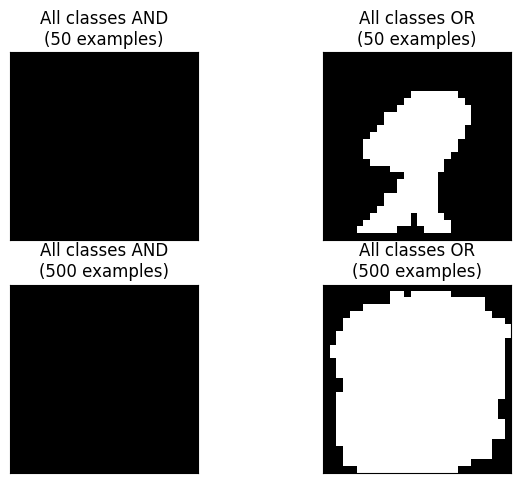
\includegraphics[width=.5\textwidth]{boolean-mask-all.png}
%     \caption{All classes mask for $\B$-relevance}
% \end{figure}

\begin{figure}[H]
    \centering
    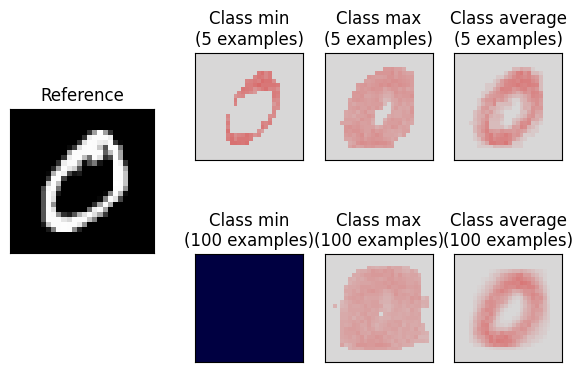
\includegraphics[width=.5\textwidth]{counting-mask.png}
    \caption{Class-wise mask for $\N$-relevance of the class \texttt{0}}
\end{figure}

\begin{figure}[H]
    \centering
    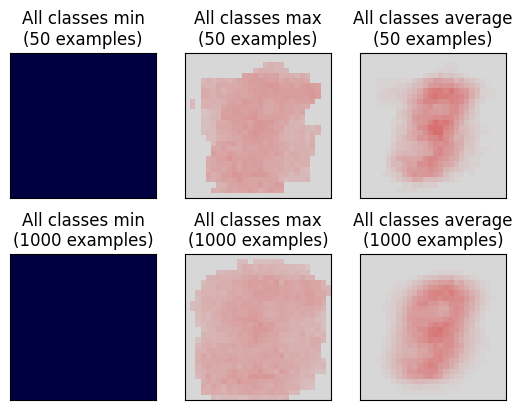
\includegraphics[width=.5\textwidth]{counting-mask-all.png}
    \caption{All classes mask for $\N$-relevance}
\end{figure}

\subsection{Network pruning using LRP ranking}
The accuracy of modern neural networks often come at the cost of large model size, increasing both storage, computational cost and inference time. To reduce the size of such models, an efficient technique called \emph{network pruning} has been studied \cite{pruning-survey,new-pruning}, in which neurons are removed from the network. A simple approach to selecting which neurons to prune is to select those with the smallest $\ell_1$ or $\ell_2$ norm: that is, those whose associated column in the weight matrix has the smallest norm. While this selection method yields good results, we show that removing neurons with the smallest average relevance -- in the sense of LRP -- allows the network to perform better.
\begin{figure}[H]
    \centering
    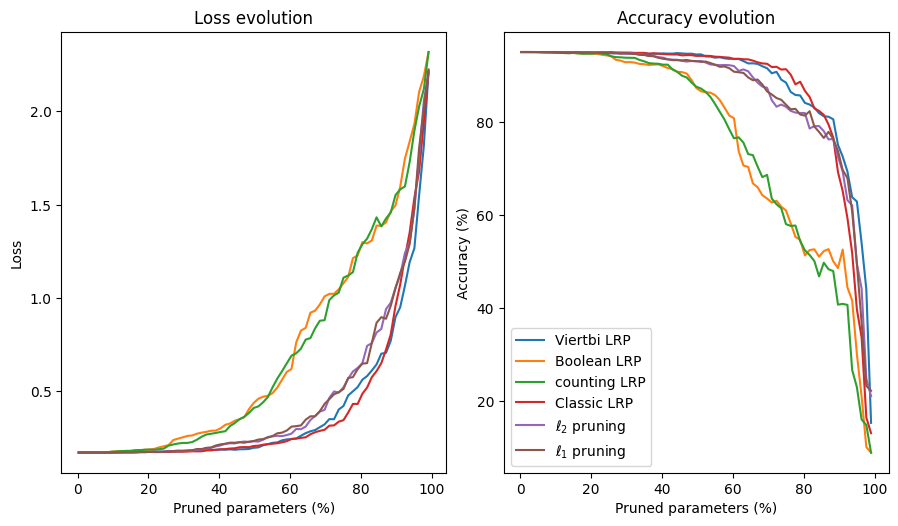
\includegraphics[width=.7\textwidth]{pruning-graph-large.png}
    \caption{Accuracy and loss evolution during network pruning for different neuron selection methods. Neurons were pruned on the first layer of the same fully-connected network trained on the MNIST dataset. Accuracy and loss are computed over the MNIST test set.}
    \label{fig:pruning-graph}
\end{figure}

\autoref{fig:pruning-graph} compares multiple selection methods. For each method, the network was evaluated multiple times on a subset of the MNIST test set, each time with an increasing number of neurons pruned, selected using the specific method. For LRP-based methods, the relevance of each neuron is computed by taking its average relevance on LRP results over images of the train set, and neurons with the lowest absolute relevance are pruned first.

Three curve clusters can be identified: boolean and counting LRP perform much worse than other selection methods, which can be explained by the lack of granularity in the explanation that these techniques provide. $\ell_1$ and $\ell_2$ norm selection methods provide a baseline to compare LRP techniques to, and both perform similarly well. Finally, classic LRP and Viterbi LRP outperform the norm-based methods by a small amount: this confirms the intuition that LRP provide a more subtle explanation than simply the magnitude of the weights connected to a neuron.

\subsection{Comparison to image perturbation}
In parallel to LRP, other methods aiming at providing a visual explanation of the decision of a classifier have emerged, such as \cite{inverting,visualizing-cnn}. An interesting approach, introduced in \cite{fong2017interpretable}, identifies pixels relevant to the classification by adding perturbations to the image. Intuitively, a pixel is relevant if the classification of the image changes when this pixel is modified. 

In \autoref{fig:mnist-attack}, we reproduced this idea by measuring the accuracy drop when different regions of the image are perturbed. Zones of the image of size $4\times4$ are modified by applying the transformation $x\longleftarrow255-x$ for pixels $x$ with values in the $\iset{0}{255}$ range. 
\begin{figure}[H]
    \centering
    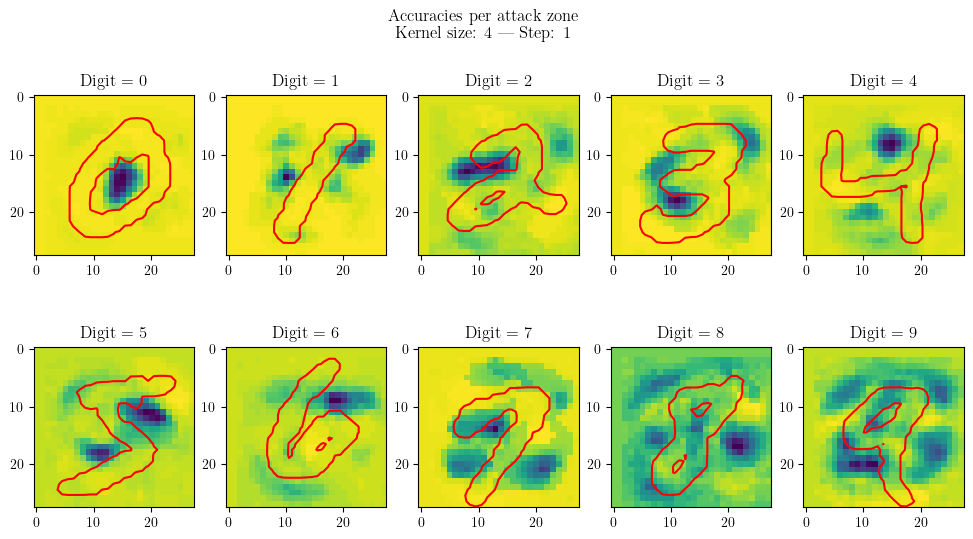
\includegraphics[width=.8\textwidth]{attacks.png}
    \caption{Accuracy sensibility to perturbation by spatial region of the image. Darker zones show drops of accuracies when this zone of the image is perturbed.}
    \label{fig:mnist-attack}
\end{figure}
This results in a visualization of the critical zones of the image, qualitatively different from LRP. While LRP highlights the zones containing the classified object, perturbation methods mostly selects zones outside of the object, where change can lead to confusion with another class: for instance, the zone above the \texttt{4} is strongly highlighted since perburbation in this area might trick the model into believing that the digit is a \texttt{9} instead.

To evaluate to what extent LRP highlights pixels vulnerable to perturbations, we studied the impact of modifications in the zones of high relevance compared to low relevance zones. To do so, we measured the accuracy of the model while progressively perturbating more and more pixels of the image. In \autoref{fig:attack-graphs}, we compare the accuracy of the model when pixels are uniformly selected in the image, to the accuracy when pixels are selected with a probability distribution depending on the relevance. If $X$ is the random variable corresponding to the pixel selected to be modified, then:
\begin{equation}
    \P(X=i) = \frac{e^{-R_i}}{\sum_je^{-R_j}}
\end{equation}
In other terms, the probability distribution is the softmax of the opposite of the relevance; the higher the relevance, the lower the probability that the pixel is affected by a perburbation.
\begin{figure}[H]
    \centering
    \begin{minipage}[c]{.49\textwidth}
        \centering
        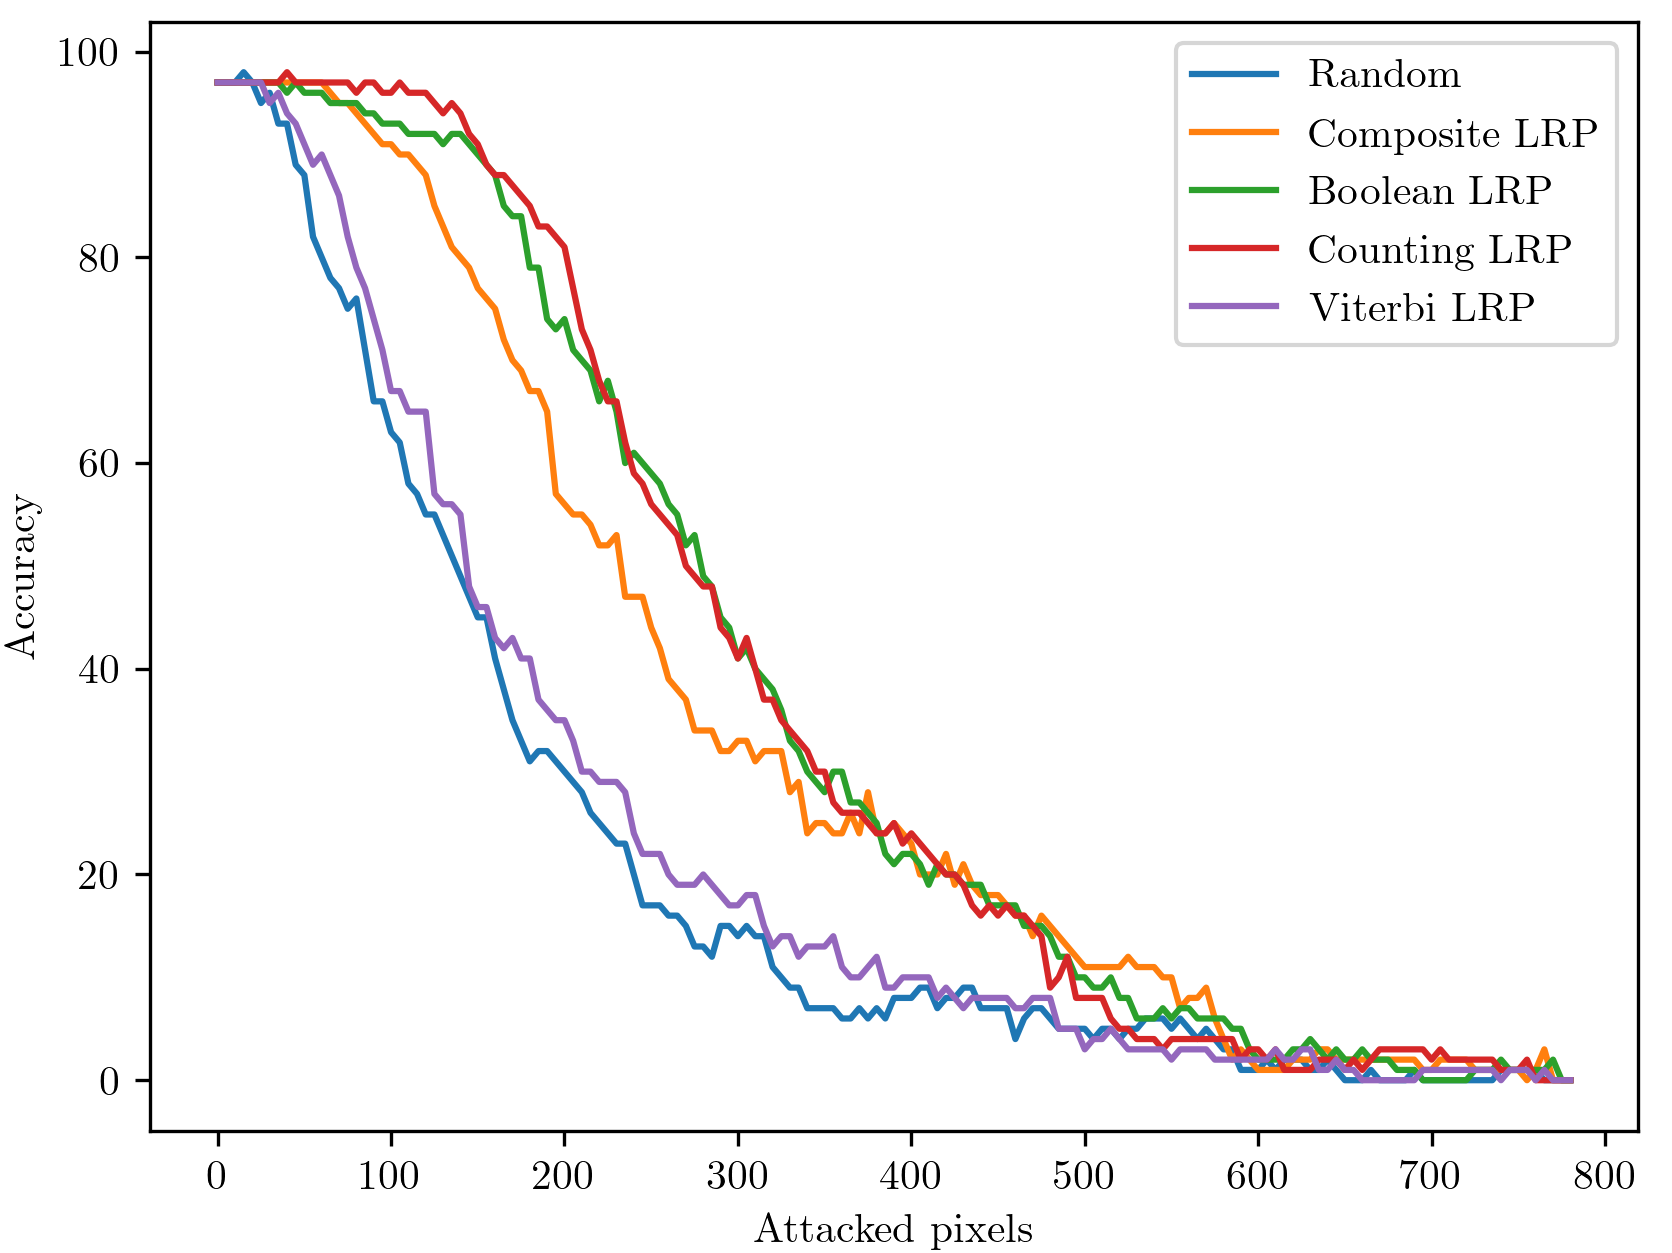
\includegraphics[width=\textwidth]{attack-graph-1.png}
    \end{minipage}
    \begin{minipage}[c]{.49\textwidth}
        \centering
        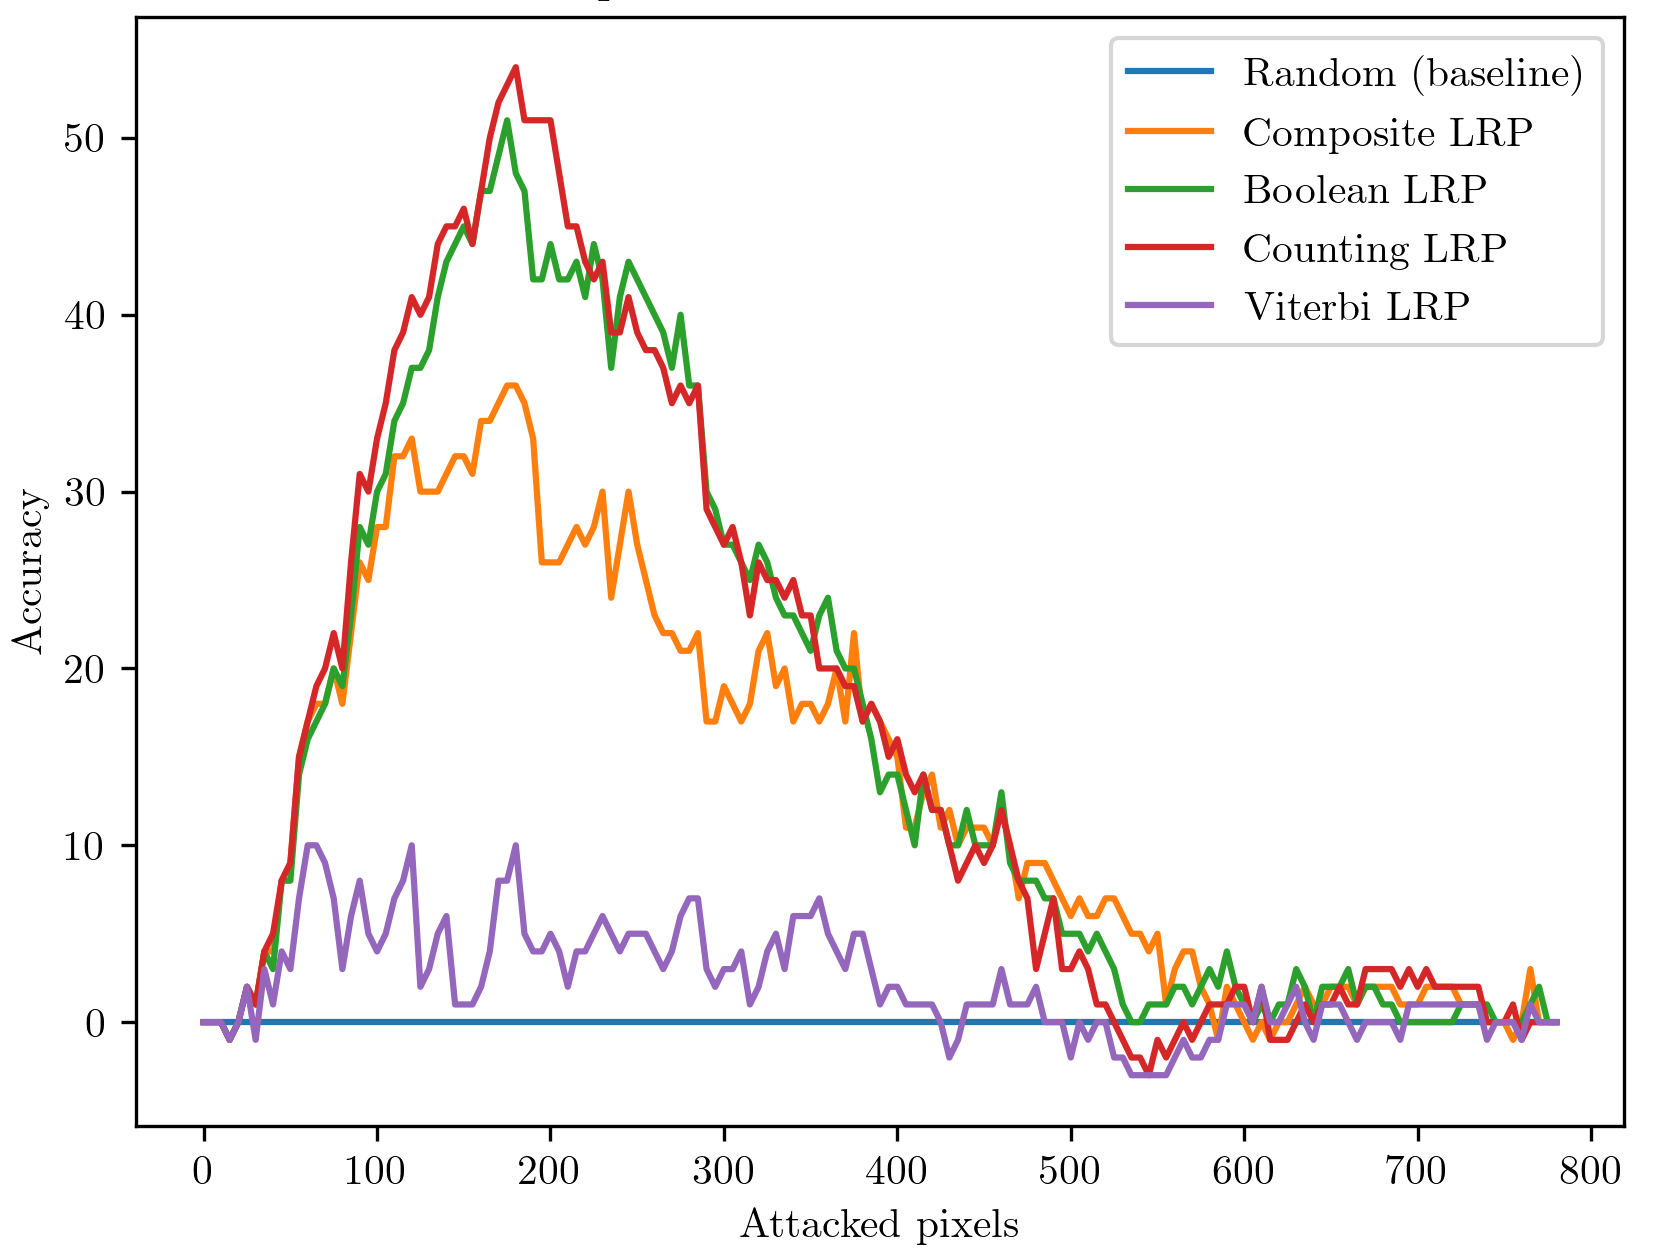
\includegraphics[width=\textwidth]{attack-graph-2.png}
    \end{minipage}
    \caption{Accuracy drop for multiple pixels attacks strategies.}
    \label{fig:attack-graphs}
\end{figure}
Results of \autoref{fig:attack-graphs} show that all LRP distributions outperform the uniform baseline. While LRP does not directly highlight vulnerable pixels, pixels with less relevance are most likely to be resilient to perturbations.

\section{Conclusion}
We introduced Semiring-based Layer-wise Relevance Propagation to extend LRP to a broader range of explanations. Semiring-based LRP benefits from the capabilities of classical LRP, while letting the user choose customized semirings for explanations that better suit the applications of its model. 

We implemented Semiring-based LRP for PyTorch models containing Linear, Convolutional, Spatial pooling, and Activation layers; the user can simply implement its own semiring by overloading the addition, multiplication, $\0$ and $\1$ elements and annotation function. Experimentally, boolean and counting semiring provide scalable explanations that qualitatively differ from classical LRP.

Finally, we explored three examples of applications of semiring-based LRP: mask computation, network pruning, and vulnerable pixels detection. We believe that semiring-based LRP has the potential to provide more than an explanation for a single execution, and those applications tend to show that combining LRP results over multiple executions produces meaningful metrics for the overall relevance of neurons in the network. 

\section*{Acknowldegements}
I would like to thank Silviu Maniu for his guidance and support throughout this internship. I thank Pierre Senellart for his feedback and advices. Thanks to the LIG and specifically to the members of the SLIDE team. In particular, thanks to Alan Gany, Nassim Bouarour for their help, and thanks to Paul Landrier for his suggestions.

\nocite{*}
\printbibliography

\newpage
\appendix

\end{document}